\documentclass[a4j,8.5pt, twocolumn,fleqn]{jbook}
\usepackage{styles/sotsu2}
\usepackage{graphicx}
\usepackage[dvipdfmx]{color}
\usepackage{styles/times}
\usepackage{enumerate}
\def\bm#1{\mbox{\boldmath $#1$}}
\表題{機械学習を用いた物損事故発生地点における人身事故発生リスクの要因分析}
\所属{\gtfamily{ 知能情報システム工学講座}}%
\著者{\gtfamily {学籍番号 1814019 近 祐大}}%
\教員{\gtfamily{ 指導教員 本吉 達郎 准教授}}%
\renewcommand\labelenumi{(\arabic{enumi})}
\begin{document}
\Atitle
\small
\vspace*{-2mm}


%%%%%%%%%%%%%%
\section{はじめに}
\subsection{人身事故予防に対する新たな取り組みの必要性}
各国における交通事故による状態別の死者数の構成比率(Fig.\ref{国別状態別30日以内死者数の構成率比較}
)によると, 日本では交通事故による死者のうち52\%が歩行中もしくは自転車乗用中である。
この割合は, Fig.\ref{国別状態別30日以内死者数の構成率比較}に示した他の国と比較して高いと言える。

また近年では, 交通事故死者,重傷者における高齢者の割合は年々増加している\cite{令和3年における交通事故の発生状況等について}。

日本では近年交通事故の発生は減少傾向にあるが、今後さらに高齢化が進行すると考えられていることや、コロナ禍による徒歩、自転車の需要の増加\cite{自転車を巡る現状等}を考慮すると, 人身事故予測・予防に対するさらなる取り組みが必要であると考えられる。

\begin{figure}[htb]
    \centering
    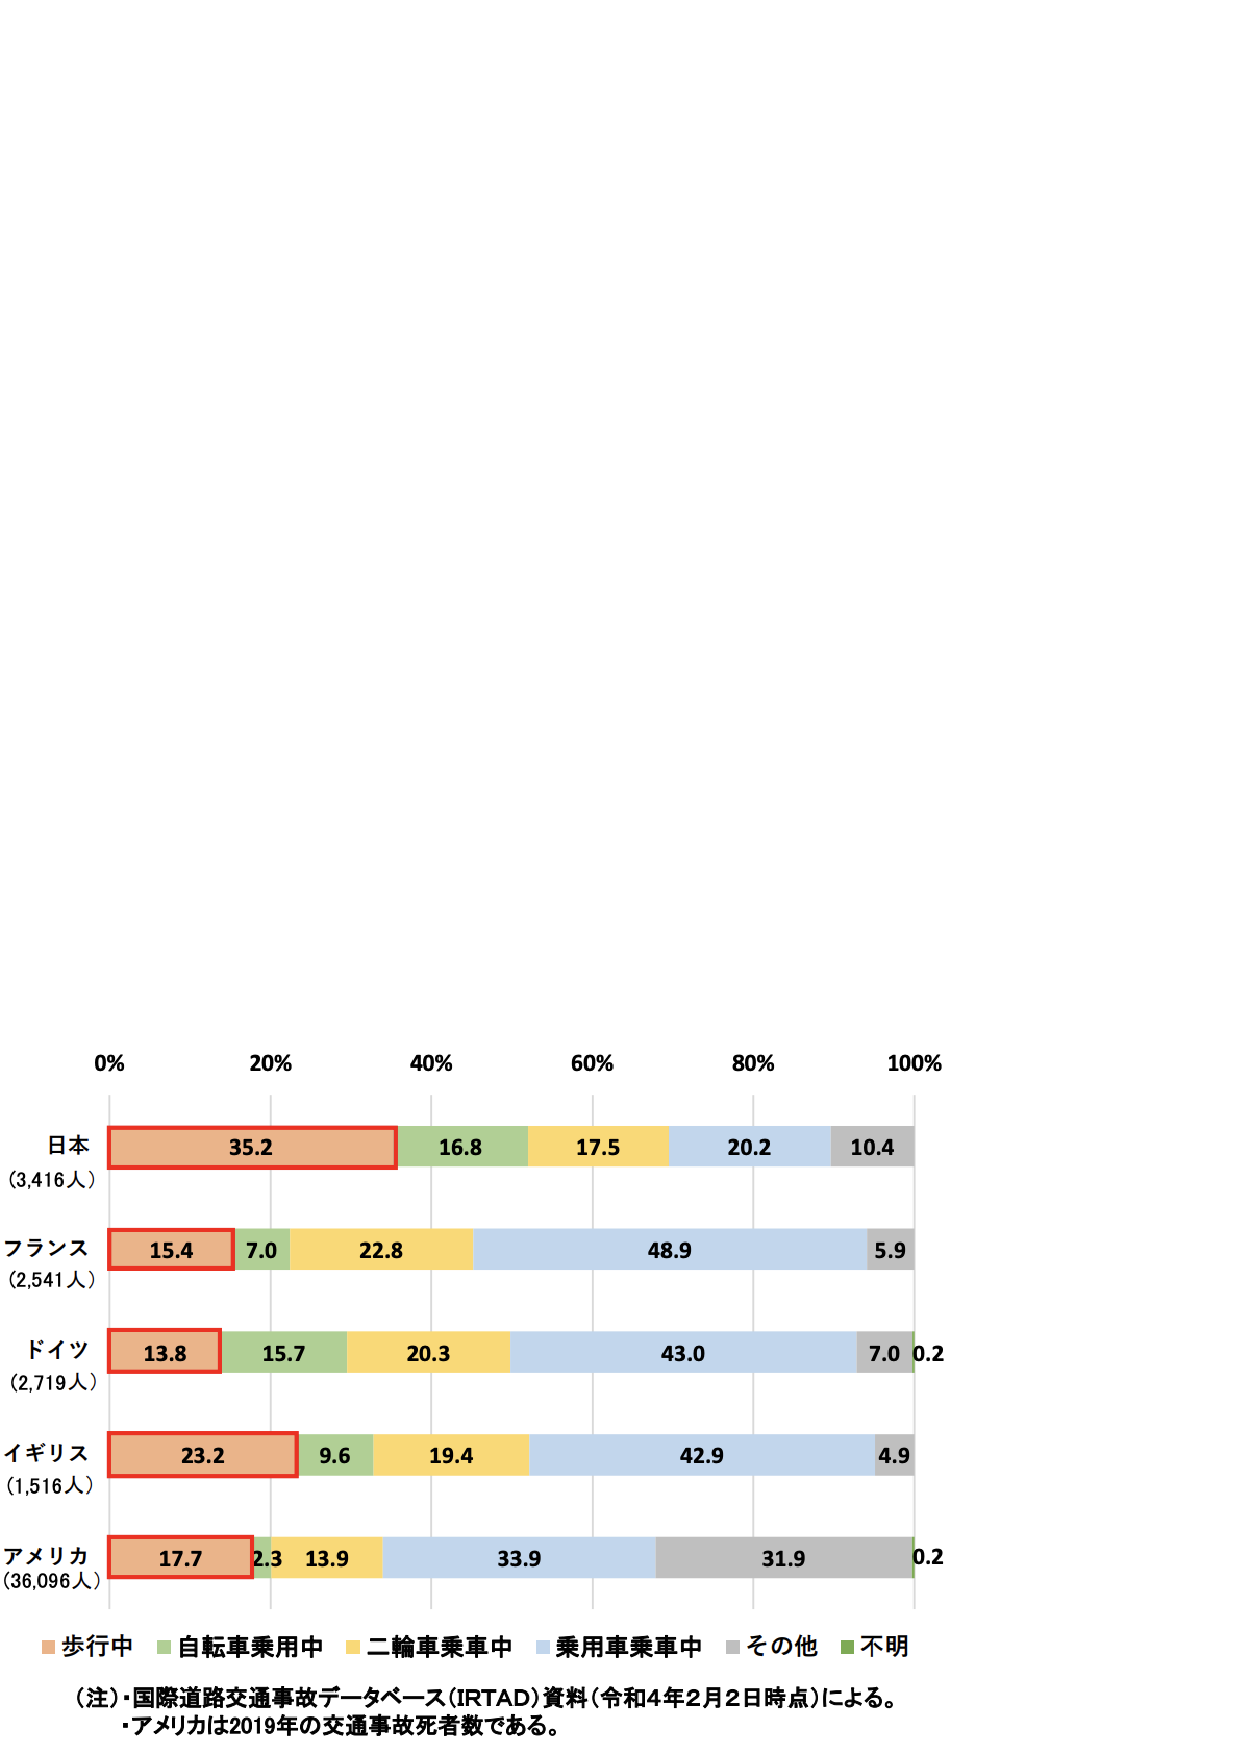
\includegraphics[height=50mm]{images/pngs/shibou_status.png}
    \vspace{-3mm}
    \caption{国別状態別30日以内死者数の構成率比較\cite{令和3年における交通事故の発生状況等について}}
    \label{国別状態別30日以内死者数の構成率比較}
\end{figure}

\subsection{人身事故予測・予防の困難性}
人身事故が発生しうる地点は無数に存在しており, 全ての地点での人身事故発生予測・予防は困難である。
このことから、交通事故が発生する可能性が高いと思われる地点を絞った上で人身事故が発生する要因を分析する手法が必要であると考えられる。

また, 人身事故の発生に影響を与えると思われる要素は無数にあり, 全ての要因を排除することは困難である。
そのため、要因排除の優先度を設定することが必要であると考えられる。

\subsection{本研究のアプローチ}
本研究では、過去に発生した交通事故データをもとに、人身事故か物損事故かを決定づける特徴を分析することで、人身事故の発生に大きな影響を与える要因を発見する手法を提案する。



%%%%%%%%%%%%%%%%%%%%
\section{本研究で用いるデータ}
本研究では, Fig.\ref{人身事故データ}に示す富山県内で発生した人身事故に関するデータ(以下人身事故データ)とFig.\ref{物損事故データ}に示す富山県内で発生した物損事故に関するデータ(以下物損事故データ)を用いる.以下、人身事故データと物損事故データを合わせて交通事故データとする。

人身事故データは平成29年から令和3年の間に富山県内で発生した人身事故に関して、道路や環境の特徴、当事者の特徴など98個の属性が記録されたものである。
物損事故データは令和3年に富山県内で発生した物損事故に関して、道路の特徴など25個の属性が記録されたものである。

なおこれらのデータは富山県警から入手したものである。

\begin{figure}[htb]
    \centering
    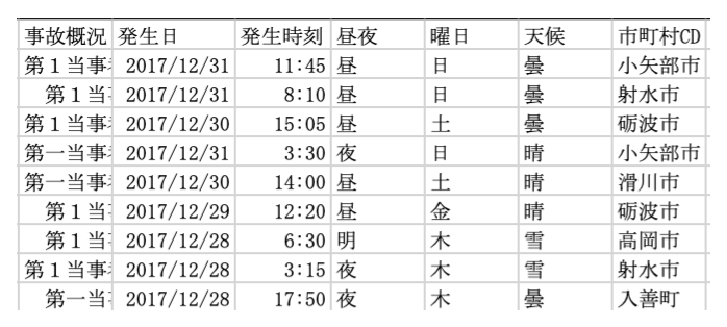
\includegraphics[height=30mm]{images/jinshixn.eps}
    \caption{人身事故データ(一部抜粋)}
    \label{人身事故データ}
\end{figure}

\begin{figure}[htb]
    \centering
    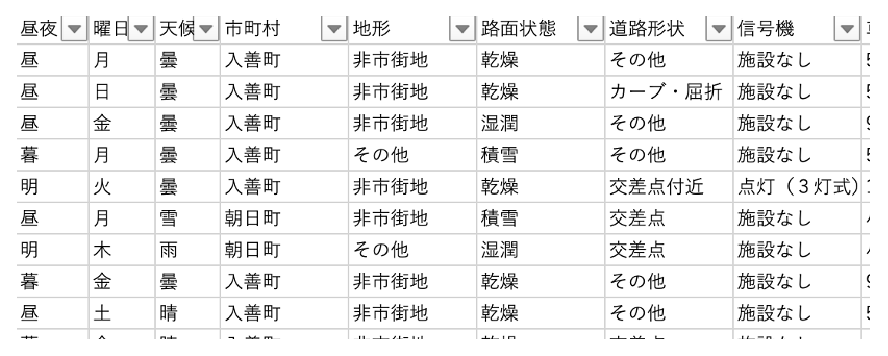
\includegraphics[height=30mm]{images/bussoxn.eps}
    \vspace{-3mm}
    \caption{物損事故データ(一部抜粋)}
    \label{物損事故データ}
\end{figure}


%%%%%%%%%%%%%%%%%%%%%
\section{本研究における分析手法}
\subsection{クラス分類}
本研究では、クラス分類を用いて交通事故の種類を決定づける特徴を分析する。
クラス分類の手法として、線形サポートベクターマシン、非線形サポートベクターマシン、勾配ブースティング決定枝が挙げられる。
複数のクラス分類手法を用いて学習を行い、本研究に用いるクラス分類手法を選定する。


\subsection{形式概念分析}
形式概念分析 ( Formal Concept Analysis )は1981年のBanff 会議"Ordered Sets"においてRudolf Wille 氏によって提案されたデータ分析手法である\cite{形式概念分析-入門・支援ソフト・応用}.
Fig.\ref{context}に示すようなデータ集合に対して形式概念分析を用いることで,共通の属性を持つオブジェクト集合と, その共通の属性集合の組み(コンセプト)を数学的に定義された概念データとして扱い,複雑なデータの構造の分析や,属性間に成り立つ含意論理の抽出によるデータ全体が持つ傾向分析を行うことが可能である。

\subsection{ImplicationとAssociation Rule}
形式概念分析では、「Aという属性を持つものは必ずBである」というルールを抽出することで、データの集合における属性間の関係を可視化する。
このルールのことをImplication(含意論理)という。動物の例におけるImplicationを\ref{implications}の番号1及び2に示す。


また形式概念分析の補助として、「Aという属性を持つオブジェクトのうち何\%はBという属性を持つ」というルールを抽出することで、外れ値によってImplicationとして出てこない属性感の関係を抽出することが可能である。
このルールのことをAssociation Rule(関連)という。動物の例におけるAssociation Ruleを\ref{implications}の番号3及び4に示す。

本研究では交通事故データにおけるAssociation Rule を抽出することで、各種類の交通事故が持つ傾向を抽出する。

\begin{figure}[htb]
    \centering
    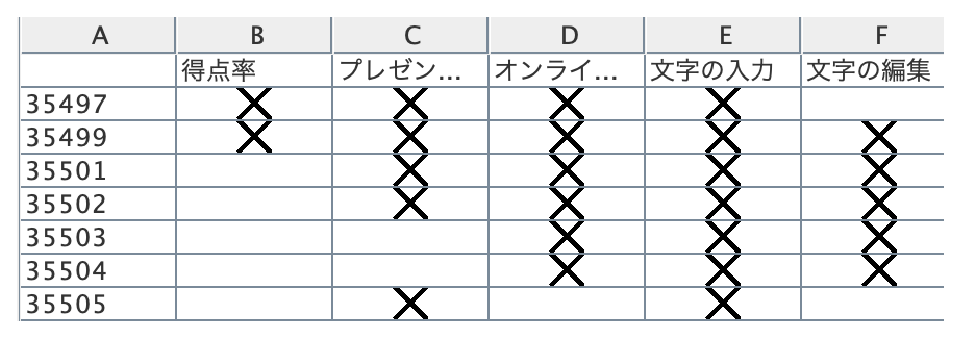
\includegraphics[height=30mm]{images/context.eps}
    \vspace{-3mm}
    \caption{動物の例におけるコンテクスト表}
    \label{context}
\end{figure}

\begin{figure}[htb]
    \centering
    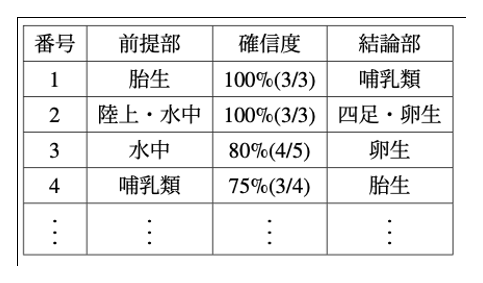
\includegraphics[height=30mm]{images/implication.eps}
    \caption{動物の例におけるImplicationとAssociation Ruleの一部}
    \label{implications}
\end{figure}


%%%%%%%%%%%%%%%%%%
\section{分析用データ収集手法}
\subsection{物損事故, 人身事故間のデータの差異}
Fig.\ref{人身事故データ}とFig.\ref{物損事故データ}に示した, 本研究で用いる人身事故データと物損事故データの間には, 記録されている属性に違いがあり、分析にあたって保有する属性を一致させる必要がある。
本研究では各事故データに対して属性を追加する手法として、座標周辺探索プログラム及び地図画像分類システムを作成した。

\subsection{座標周辺探索プログラム}
本プログラムでは、国土交通省の国土数値情報ダウンロードサービス\cite{国土数値情報ダウンロードサービス}より入手した各施設に関する外部データを用いて、交通事故発生地点周辺に特定の施設の存在を判定する。

本プログラムを用いて交通事故発生地点が小学校や都市公園などの施設の周辺であるかどうかを属性として保存する。

\subsection{地図画像分類システム}
本システムでは, 道路線形や道路形状, 信号の有無などを機械学習を用いて物損事故データに追加する。Fig.\ref{classifications}に簡易的なサーバ構成を示す。

本システムは、地図画像取得および整形用スクリプト配布サーバ(以下WebAPサーバ)と、タイル画像配布サーバ(以下地図配布サーバ)によって構成される。
WebAPサーバはJavaプラットフォーム向けのフレームワークであるSpringBoot\cite{literature3}を用いて作成し, 地図配布サーバにはリクエストに応じて環境内のタイル画像データベースより地図の画像を送信する機能を持つオープンソースソフトウェアであるmbtile-server\cite{literature4}を用いた。
今回は地図画像データベースとして、ダウンロード及び個人利用が許可されている"OpenMapTiles"と"地理院タイル"を用いた。
本システムを用いて取得した交通事故発生地点周辺地図の例をFig.\ref{tiriixn}に示す。

\begin{figure}[htb]
    \centering
    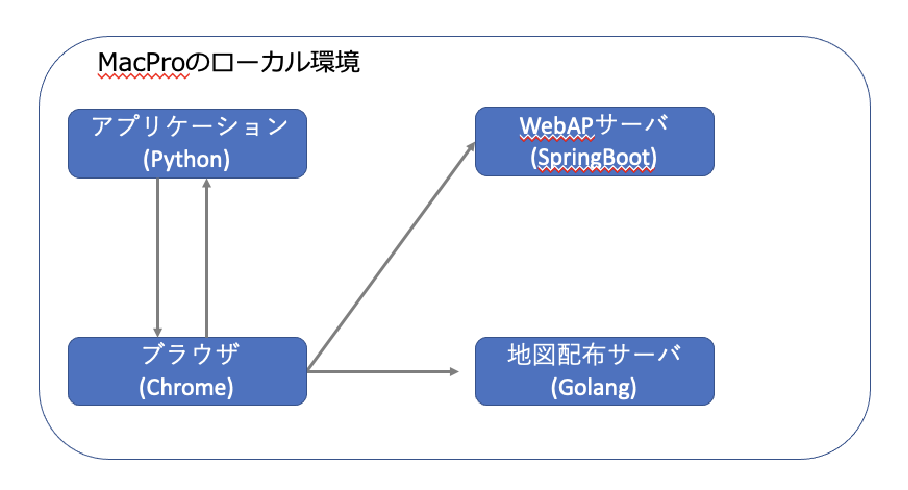
\includegraphics[height=30mm]{images/mapclassification_server.eps}
    \vspace{-3mm}
    \caption{地図画像分類システム}
    \label{classifications}
\end{figure}

\begin{figure}[htb]
    \centering
    
\includegraphics[height=30mm]{images/tiriixn.eps}
    \vspace{-3mm}
    \caption{交通事故発生地点周辺地図の例}
    \label{tiriixn}
\end{figure}

本システムでは, Pythonで記述された画像分類アプリケーションがブラウザを介して物損事故発生地点周辺の地図画像を取得して, 人身事故データを用いて学習した結果をもとに物損事故発生地点の情報を追加する。

%%%%%%%%%%%%%%%%%%%%%
\section{分析用データ収集の結果}
\subsection{座標周辺探索プログラムによるデータ収集の結果}
国土数値情報ダウンロードシステムの"小学校区(ポリゴン)を用いて交通事故発生地点周辺の小学校の有無を判定し、交通事故データに追加した。

人身事故発生地点のうち小学校周囲100m以内と判定された地点の地図(Google Map)をFig.\ref{shougakkou_gmap}に示す。

\begin{figure}[htb]
    \centering
    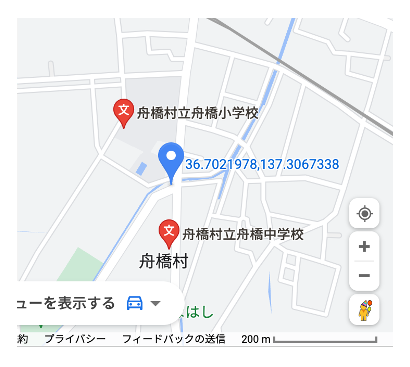
\includegraphics[height=30mm]{images/shougakkou_gmap.eps}
    \vspace{-3mm}
    \caption{小学校周辺の交通事故発生地点の例}
    \label{shougakkou_gmap}
\end{figure}

\subsection{地図画像分類システムによるデータ追加の結果}
構築した地図画像分類システムを用いて交通事故データの座標に対して道路上か道路以外か分類した。
人身事故データを用いた学習の結果をTable.\ref{table_road}に示す。


\begin{table}[htb]
    \centering
    \caption{交通事故発生位置に対する学習の結果}
    \label{table_road}
    \begin{tabular}{|l|l|}
        \hline
        \textbf{データの種類} & \textbf{正解率} \\ \hline
        道路上で発生した事故データ   & 0.8942       \\ \hline
        道路外で発生した事故データ   & 0.9016       \\ \hline
        全体の事故データ        & 0.8945       \\ \hline
    \end{tabular}
\end{table}

%%%%%%%%%%%%%
\section{まとめ}
本研究では、過去に物損事故が発生した地点において人身事故発生リスクの要因を分析する手法として、交通事故データに対してクラス分類を行う手法を提案する。

交通事故データに対してクラス分類を行う上で、人身事故及び物損事故発生地点に関する特徴を追加するツールを作成した。

今後の作業として、作成したツールを用いたデータ収集と、収集したデータを用いて作成した交通事故データに対してクラス分類を行い、人身事故と判定されるデータに共通する特徴を抽出し、形式概念分析を用いて抽出された特徴がAssociation Ruleとして抽出されることを確認する。

\begin{thebibliography}{9}
    \bibitem{令和3年における交通事故の発生状況等について}警察庁交通局,令和3年における交通事故の発生状況等について, 2022
    \bibitem{自転車を巡る現状等}国土交通省, 令和2年度第2回自転車の活用推進に向けた有識者会議 / 自転車を巡る現状等【参考資料】
    \bibitem{形式概念分析-入門・支援ソフト・応用}鈴木治,室伏俊明,形式概念分析-入門・支援ソフト・応用-,日本知能情報ファジィ学会誌,Vol.19, No.2, pp.103-142, 2007
    \bibitem{国土数値情報ダウンロードサービス}国土交通省, 国土数値情報ダウンロードサービス, [https://nlftp.mlit.go.jp/ksj/], (2022/11/14)
    \bibitem{literature3}Spring Boot, [https://spring.io/projects/spring-boot], (2022/11/14)
    \bibitem{literature4}consbio, mbtileserver, [https://github.com/consbio/mbtileserver], (2022/11/14)
\end{thebibliography}


\end{document}

